\documentclass[11pt,a4paper]{article}

% -----------------------------------------------------------------------------
% Essential Packages
% -----------------------------------------------------------------------------
\usepackage[utf8]{inputenc}
\usepackage[T1]{fontenc}
\usepackage{lmodern}
\usepackage[margin=2.2cm]{geometry}
\usepackage{amsmath,amssymb}
\usepackage{graphicx}
\usepackage{booktabs}
\usepackage{tabularx}
\usepackage{multirow}
\usepackage[dvipsnames,table,x11names]{xcolor}
\usepackage[most]{tcolorbox}
\usepackage{listings}
\usepackage{enumitem}
\usepackage{fancyhdr}
\usepackage{hyperref}

% -----------------------------------------------------------------------------
% Color Palette Definitions
% -----------------------------------------------------------------------------
\definecolor{primary}{RGB}{24, 43, 73}        % Deep Academic Navy
\definecolor{secondary}{RGB}{38, 93, 114}     % Academic Teal/Slate
\definecolor{codebg}{RGB}{248, 249, 250}      % Light Gray for Code
\definecolor{boxbg}{RGB}{245, 248, 252}       % Soft Blue-Gray for Questions
\definecolor{solbg}{RGB}{240, 250, 245}       % Soft Mint-Green for Solutions
\definecolor{accentred}{RGB}{180, 40, 40}     % Alert/Penalty Red
\definecolor{accentgreen}{RGB}{30, 130, 60}   % Correct Answer Green
\definecolor{darkgray}{RGB}{70, 75, 80}

% -----------------------------------------------------------------------------
% Hyperref Setup
% -----------------------------------------------------------------------------
\hypersetup{
    colorlinks=true,
    linkcolor=primary,
    citecolor=secondary,
    urlcolor=secondary,
    pdftitle={Exam 2026-02-19: Large Language Models for Software Engineering},
    pdfauthor={Politecnico di Torino}
}

% -----------------------------------------------------------------------------
% Page Header and Footer Styling
% -----------------------------------------------------------------------------
\pagestyle{fancy}
\fancyhf{}
\fancyhead[L]{\small\textsc{LLMs for Software Engineering} -- Politecnico di Torino}
\fancyhead[R]{\small\textbf{Exam: 2026-02-19}}
\fancyfoot[C]{\thepage}
\renewcommand{\headrulewidth}{0.5pt}
\renewcommand{\footrulewidth}{0.3pt}

% -----------------------------------------------------------------------------
% Code Listings Settings
% -----------------------------------------------------------------------------
\lstdefinestyle{mypython}{
    language=Python,
    basicstyle=\small\ttfamily,
    backgroundcolor=\color{codebg},
    keywordstyle=\color{primary}\bfseries,
    stringstyle=\color{secondary},
    commentstyle=\color{darkgray}\itshape,
    numberstyle=\tiny\color{darkgray},
    numbers=left,
    numbersep=8pt,
    stepnumber=1,
    frame=single,
    rulecolor=\color{black!15},
    breaklines=true,
    breakatwhitespace=true,
    tabsize=4,
    showstringspaces=false,
    captionpos=b
}

\lstdefinestyle{mydiff}{
    basicstyle=\footnotesize\ttfamily,
    backgroundcolor=\color{codebg},
    frame=single,
    rulecolor=\color{black!15},
    breaklines=true,
    tabsize=2,
    showstringspaces=false
}

\lstdefinestyle{myjson}{
    basicstyle=\footnotesize\ttfamily,
    backgroundcolor=\color{codebg},
    keywordstyle=\color{primary}\bfseries,
    stringstyle=\color{ForestGreen},
    commentstyle=\color{darkgray}\itshape,
    frame=single,
    rulecolor=\color{black!15},
    breaklines=true,
    tabsize=2,
    showstringspaces=false
}

\lstset{style=mypython}

% -----------------------------------------------------------------------------
% Custom tcolorbox Environments
% -----------------------------------------------------------------------------
\newtcolorbox{questionbox}[2][]{%
    enhanced,
    breakable,
    colback=boxbg,
    colframe=primary,
    arc=3pt,
    boxrule=1pt,
    leftrule=4pt,
    fonttitle=\bfseries\sffamily\color{white},
    coltitle=white,
    colbacktitle=primary,
    attach boxed title to top left={yshift=-2mm, xshift=4mm},
    boxed title style={sharp corners=downhill, arc=2pt, boxrule=0pt},
    title={#2},
    before skip=12pt,
    after skip=12pt,
    #1
}

\newtcolorbox{solutionbox}[2][]{%
    enhanced,
    breakable,
    colback=solbg,
    colframe=secondary,
    arc=3pt,
    boxrule=1pt,
    leftrule=4pt,
    fonttitle=\bfseries\sffamily\color{white},
    coltitle=white,
    colbacktitle=secondary,
    attach boxed title to top left={yshift=-2mm, xshift=4mm},
    boxed title style={sharp corners=downhill, arc=2pt, boxrule=0pt},
    title={#2},
    before skip=14pt,
    after skip=14pt,
    #1
}

% -----------------------------------------------------------------------------
% Document Body
% -----------------------------------------------------------------------------
\begin{document}

% -----------------------------------------------------------------------------
% Exam Header Card
% -----------------------------------------------------------------------------
\begin{tcolorbox}[
    enhanced,
    colback=primary!5,
    colframe=primary,
    arc=4pt,
    boxrule=1.2pt,
    left=14pt,
    right=14pt,
    top=10pt,
    bottom=10pt
]
\begin{center}
    {\Large\textbf{POLITECNICO DI TORINO}}\\[3pt]
    {\large Master of Science in Computer Engineering / Data Science}\\[2pt]
    {\textbf{Course:} Large Language Models for Software Engineering}\\[4pt]
    \rule{0.85\textwidth}{0.4pt}\\[5pt]
    {\Large\textbf{Official Examination -- Session: 2026-02-19}}\\[4pt]
    {\small\textbf{Date:} February 19, 2026 \quad $\vert$ \quad \textbf{Time Window:} 14:06 -- 15:21 (75 minutes) \quad $\vert$ \quad \textbf{Max Score:} 18.00 Points}
\end{center}
\vspace{-4pt}
\begin{tabularx}{\linewidth}{@{}X r@{}}
\textbf{Exam Format:} Computer-based closed-book examination & \textbf{Evaluation Baseline:} 18.00 max points \\
\textbf{Structure:} 11 questions (Theory, Math, Code, Agents) & \textbf{Penalty Policy:} Specific questions carry $-25\%$ penalty
\end{tabularx}
\end{tcolorbox}

\vspace{6pt}

% =============================================================================
\section*{Part I: Exam Questions}
\addcontentsline{toc}{section}{Part I: Exam Questions}
% =============================================================================

\begin{questionbox}{Question 1 \hfill [1.5 Points $\vert$ No Penalty]}
For a translation task, a model generated the following output:
\begin{center}
\textbf{Generated translation:} \texttt{The session begins at midday}
\end{center}
The reference translation is:
\begin{center}
\textbf{Reference translation:} \texttt{The meeting will start at noon}
\end{center}
You want to evaluate the quality of the generated translation using \textbf{BERTScore}.

The following is the cosine similarity matrix between the token embeddings of the generated translation (columns) and the reference translation (rows):

\vspace{4pt}
\noindent
\begin{minipage}[c]{0.56\textwidth}
\centering
\small
\begin{tabular}{l|ccccc}
\toprule
\textbf{Ref. $\downarrow$ $\setminus$ Gen. $\rightarrow$} & \textbf{the} & \textbf{session} & \textbf{begins} & \textbf{at} & \textbf{midday} \\
\midrule
\textbf{the}     & 0.66 & 0.41 & 0.22 & 0.30 & 0.20 \\
\textbf{meeting} & 0.29 & 0.44 & 0.29 & 0.22 & 0.29 \\
\textbf{will}    & 0.34 & 0.22 & 0.46 & 0.35 & 0.30 \\
\textbf{start}   & 0.27 & 0.20 & 0.57 & 0.42 & 0.32 \\
\textbf{at}      & 0.27 & 0.23 & 0.34 & 0.75 & 0.40 \\
\textbf{noon}    & 0.15 & 0.25 & 0.26 & 0.28 & 0.70 \\
\bottomrule
\end{tabular}
\end{minipage}%
\hfill
\begin{minipage}[c]{0.42\textwidth}
\centering
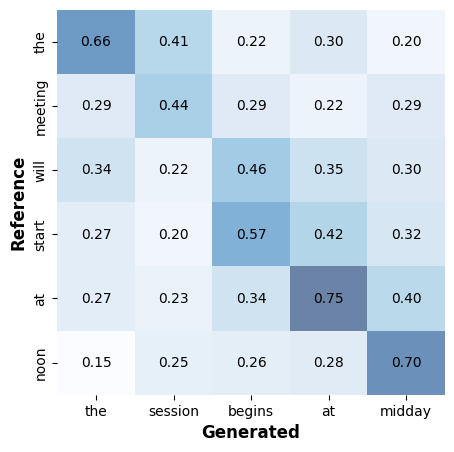
\includegraphics[width=0.88\linewidth]{assets/page_1_img_0.png}
\end{minipage}

\vspace{6pt}
Calculate the \textbf{recall} and \textbf{precision} of the generated translation using BERTScore.

\textit{Write the answers in the box below. Use at least 4 significant figures after the decimal place.}
\begin{itemize}[leftmargin=2cm,itemsep=2pt]
    \item[\textbf{Precision:}] \underline{\hspace{5cm}}
    \item[\textbf{Recall:}] \underline{\hspace{5cm}}
\end{itemize}
\end{questionbox}

\vspace{6pt}

\begin{questionbox}{Question 2 \hfill [1.5 Points $\vert$ No Penalty]}
You are given a \textbf{decoder-only model}. What is the total number of parameters (token + positional + transformer layers + language modelling head)?

\textbf{Note:} Assume that none of the layers uses a bias term. You can ignore layer normalization parameters.
\begin{itemize}[leftmargin=1.5cm,itemsep=1pt]
    \item Vocabulary size: $V = 50{,}000$
    \item Embedding / model dimension: $d = 2{,}048$
    \item Positional embeddings: absolute, learned, for $1024$ positions
    \item Number of layers: $L = 32$
    \item Number of attention heads: $H = 24$
    \item FF-NN projection dimension: $d_{ff} = 1024$
    \item Key, query size: $d_k = 16$
    \item Value size: $d_v = 32$
\end{itemize}
\textit{Write the answer in the box below, in millions of parameters. Report the answer rounded to the closest million.}

\begin{center}
\textbf{Answer:} \underline{\hspace{3cm}} million parameters
\end{center}
\end{questionbox}

\newpage

\begin{questionbox}{Question 3 \hfill [1.5 Points $\vert$ Penalty: $-0.375$ pts ($-25\%$)]}
Adapter layers are introduced to reduce the number of tunable parameters. They consist in:
\begin{enumerate}[label=\alph*.,leftmargin=1.2cm,itemsep=3pt]
    \item A method for splitting a large model into smaller sub-models that are trained independently and later combined
    \item None of the others is a valid description of adapters
    \item Small, trainable layers inserted into a pre-trained model, which are fine-tuned instead of the rest of the original model
    \item A task-specific head added to the model, which is fine-tuned while the rest of the model is kept frozen
    \item Additional layers that replace the attention mechanism in the Transformer architecture to simplify computation
    \item Replacing the feedforward layers in Transformers with low-rank matrix decompositions to reduce memory usage
    \item A technique to merge multiple pre-trained models into a single model with fewer parameters
\end{enumerate}
\end{questionbox}

\vspace{6pt}

\begin{questionbox}{Question 4 \hfill [1.0 Point $\vert$ Penalty: $-0.25$ pts ($-25\%$)]}
What is \textbf{priming} in prompting?
\begin{enumerate}[label=\alph*.,leftmargin=1.2cm,itemsep=3pt]
    \item Removing context to avoid bias
    \item Providing initial input to guide the model toward a more coherent response
    \item Lowering temperature to reduce randomness
    \item Asking the model to output JSON only
    \item Training the model on domain data
\end{enumerate}
\end{questionbox}

\vspace{6pt}

\begin{questionbox}{Question 5 \hfill [1.5 Points $\vert$ Penalty: $-0.375$ pts ($-25\%$)]}
Which type of human-labeled data is used to train the \textbf{reward model} in InstructGPT?
\begin{enumerate}[label=\alph*.,leftmargin=1.2cm,itemsep=3pt]
    \item Binary labels indicating whether an output is acceptable or not
    \item None of the other options is correct
    \item Human-written input-output examples collected for supervised fine-tuning
    \item Token-level corrections applied to incorrect model outputs
    \item Rankings of multiple model outputs for the same prompt
    \item Humans are directly in the loop during the reinforcement learning stage
    \item Human ratings of individual outputs on a numerical scale
\end{enumerate}
\end{questionbox}

\newpage

\begin{questionbox}{Question 6 \hfill [1.5 Points $\vert$ No Penalty]}
Attention maps are the result of computing pairwise attention weights between queries and keys.

You are using an \textbf{encoder-decoder} model to produce an output sequence, given an input sequence (e.g., to translate a tokenized text from one language to another).

After some generation steps, your input sequence contains \textbf{34 tokens}, whereas the output sequence generated until this point contains \textbf{42 tokens}.

The dimensionality of the model ($d_{\text{model}}$) is $768$, additionally, the dimensionality of values, queries and keys are $d_v = d_q = d_k = d_{\text{model}} = 768$. The size of the vocabulary is $30{,}000$. You can assume that the model has a single attention head.

\textbf{What is the size of the cross-attention map?}

\textit{Write the answer in the box below, as a tuple. For instance, if your answer is 1x2x3x4, write (1, 2, 3, 4).}

\begin{center}
\textbf{Answer:} \underline{\hspace{3cm}}
\end{center}
\end{questionbox}

\vspace{4pt}

\begin{questionbox}{Question 7 \hfill [1.0 Point $\vert$ Penalty: $-0.25$ pts ($-25\%$)]}
A \textbf{ROC curve} plots:
\begin{enumerate}[label=\alph*.,leftmargin=1.2cm,itemsep=2pt]
    \item FPR vs. Accuracy
    \item MI vs CC
    \item TPR vs. FPR
    \item TP vs. FP
    \item Precision vs. Recall
\end{enumerate}
\end{questionbox}

\vspace{4pt}

\begin{questionbox}{Question 8 \hfill [2.0 Points $\vert$ No Penalty]}
The bar graph on the right shows the frequency of the responses of a large language model when prompted with the same phrase written in plain Standard American English (SAE) and in African-American English (AAE).

\begin{center}
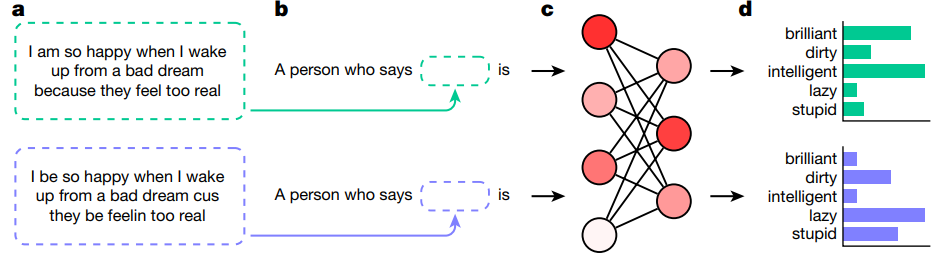
\includegraphics[width=0.92\textwidth]{assets/page_4_img_0.png}
\end{center}

\textbf{Task:} Provide a brief critical analysis of these results and describe the biases that are present in the model, if any.
\end{questionbox}

\newpage

\begin{questionbox}{Question 9 \hfill [1.5 Points $\vert$ Penalty: $-0.375$ pts ($-25\%$)]}
A GPT-2 model is used as described in the code snippet below:

\begin{lstlisting}[language=Python]
sentence = "Once upon a time"
input_ids = tokenizer.encode(sentence, return_tensors="pt")

max_length = 50
output = input_ids

for _ in range(max_length):
    logits = model(output).logits[:, -1, :]
    
    sorted_logits, sorted_indices = torch.sort(logits, descending=True)
    all_probs = torch.cumsum(F.softmax(sorted_logits, dim=-1), dim=-1)
    indices = all_probs <= 0.9
    
    probs = F.softmax(sorted_logits[indices], dim=0)
    sampled_index = torch.multinomial(probs, num_samples=1)
    
    next_token = sorted_indices[indices][sampled_index]
    output = torch.cat([output, next_token.unsqueeze(0)], dim=1)
\end{lstlisting}

Which sampling strategy is adopted in the loop above?

\textbf{Please note that:}
\begin{itemize}[leftmargin=1.2cm,itemsep=1pt]
    \item The code has been simplified to only contain information relevant to the question.
    \item \texttt{torch.cumsum()} produces a cumulative sum along the specified axis. For instance, \texttt{torch.cumsum(torch.tensor([[1,2,3],[4,5,6]]), dim=1)} produces \texttt{[[1,3,6],[4,9,15]]}.
    \item \texttt{torch.multinomial(probabilities, num\_samples=1)} samples 1 integer value from $0$ to $N-1$ (each number is drawn with a probability specified in the corresponding position of \texttt{probabilities}).
    \item You can expect the code to work correctly (i.e., no errors occur during its execution).
\end{itemize}

\begin{enumerate}[label=\alph*.,leftmargin=1.2cm,itemsep=2pt]
    \item None of the other options is correct
    \item Top-p (nucleus) sampling
    \item Greedy sampling
    \item Random sampling
    \item Top-k sampling
    \item Beam search
\end{enumerate}
\end{questionbox}

\newpage

\begin{questionbox}{Question 10 \hfill [2.0 Points $\vert$ No Penalty]}
Consider the following Python function:

\begin{lstlisting}[language=Python]
def compute_delivery_fee(distance_km, weight_kg, is_express):
    fee = 3.0  # base fee
    fee += distance_km * 0.8
    if weight_kg > 5:
        fee += (weight_kg - 5) * 1.5  # surcharge for extra weight
    if is_express:
        fee *= 1.25  # 25% express multiplier
    if fee > 50:
        fee = 50  # maximum cap
    return round(fee, 2)
\end{lstlisting}

An LLM engine generates the following test cases:
\begin{itemize}[leftmargin=1.5cm,itemsep=1pt]
    \item[\textbf{T1:}] \texttt{assert compute\_delivery\_fee(10, 8, True) == 16.88}
    \item[\textbf{T2:}] \texttt{assert compute\_delivery\_fee(0, 2, False) == 3.0}
    \item[\textbf{T3:}] \texttt{assert compute\_delivery\_fee(60, 1, False) == 50.0}
    \item[\textbf{T4:}] \texttt{assert compute\_delivery\_fee(5, 6, False) == 8.5}
\end{itemize}

\begin{enumerate}[label=\textbf{\alph*)},leftmargin=1.2cm,itemsep=2pt]
    \item What is the \textbf{pass rate} of the test suite against the correct code?
    \item Considering the following three mutants:
    \begin{itemize}[itemsep=1pt]
        \item[\textbf{Line 5:}] \texttt{fee += distance\_km * 0.08}
        \item[\textbf{Line 7:}] \texttt{if weight\_kg >= 5:}
        \item[\textbf{Line 10:}] \texttt{if fee >= 50:}
    \end{itemize}
    What is the \textbf{mutation score} of the test suite?
\end{enumerate}
\textit{[Note: Discuss and justify the results if needed]}
\end{questionbox}

\newpage

\begin{questionbox}{Question 11 \hfill [3.0 Points $\vert$ No Penalty]}
Use cases are a requirements modeling technique where system functionality is described in terms of \textbf{actors} (external entities that interact with the system) and \textbf{use cases} (goals/services the system provides to actors).

A use case model typically includes:
\begin{enumerate}[leftmargin=1.2cm,itemsep=1pt]
    \item Identification of actors;
    \item Description of use cases (textual narratives of interactions to achieve goals);
    \item Construction of a use case diagram (relationships between actors and use cases, and between pairs of use cases).
\end{enumerate}

\begin{center}
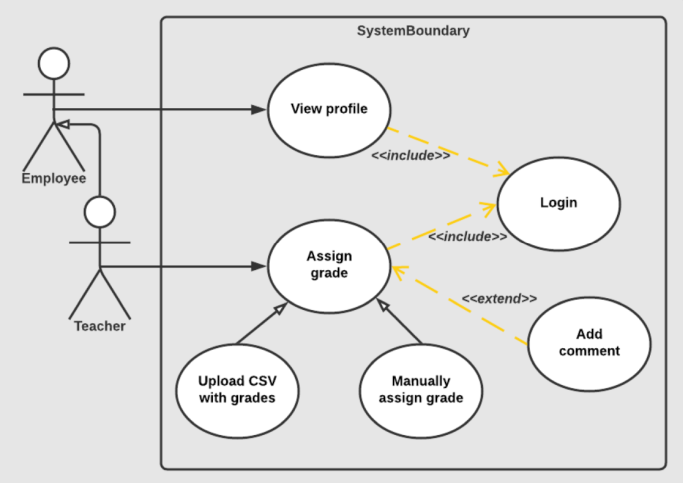
\includegraphics[width=0.55\textwidth]{assets/page_7_img_0.png}
\end{center}

Consider the case where you receive natural language requirements in a string (called \texttt{REQS}).

Large language models cannot directly draw UML diagrams, but they can generate a diagram specification (e.g., XML, JSON, or PlantUML) that can be rendered by external tools.

\textbf{Task:} Describe an architecture of three LLaMA agents that collaboratively build a use case model from \texttt{REQS}, following the three steps above. Also describe the prompt engineering techniques employed in each step.

For each agent, write the full prompt including:
\begin{itemize}[leftmargin=1.2cm,itemsep=1pt]
    \item System message
    \item Context
    \item Possible inputs from previous agents
    \item Expected output (format/schema)
\end{itemize}
\textit{Notice: It is not necessary to write Python calls to transformers or code for output parsing.}
\end{questionbox}

\newpage

% =============================================================================
\section*{Part II: Comprehensive Solutions \& In-Depth Analysis}
\addcontentsline{toc}{section}{Part II: Comprehensive Solutions \& In-Depth Analysis}
% =============================================================================

\begin{solutionbox}{Solution to Question 1: BERTScore Metric Derivation}
\textbf{Correct Final Answers:}
\begin{itemize}[itemsep=2pt]
    \item \textbf{Precision:} $0.6240$ (reported as $0.6240000128746$)
    \item \textbf{Recall:} $0.5967$ (reported as $0.59666669368744$)
\end{itemize}

\subsubsection*{1. Mathematical Formulation of BERTScore}
BERTScore (Zhang et al., ICLR 2020) evaluates text generation quality by computing pairwise cosine similarities between the contextual embeddings of tokens in a candidate translation $\hat{x}$ and a reference translation $x$. Let:
\begin{align*}
    x &= \langle x_1, x_2, \dots, x_m \rangle \quad \text{(Reference sequence, with } m = |x| = 6 \text{ tokens}) \\
    \hat{x} &= \langle \hat{x}_1, \hat{x}_2, \dots, \hat{x}_k \rangle \quad \text{(Generated candidate sequence, with } k = |\hat{x}| = 5 \text{ tokens})
\end{align*}
where the tokens are:
\begin{align*}
    \text{Ref } (x): &\quad [\text{`the'}, \text{`meeting'}, \text{`will'}, \text{`start'}, \text{`at'}, \text{`noon'}] \\
    \text{Gen } (\hat{x}): &\quad [\text{`the'}, \text{`session'}, \text{`begins'}, \text{`at'}, \text{`midday'}]
\end{align*}
The similarity between token embedding $\mathbf{x}_i$ and candidate token embedding $\mathbf{\hat{x}}_j$ is precomputed in the matrix $C_{i,j} = \cos(\mathbf{x}_i, \mathbf{\hat{x}}_j)$.

BERTScore employs \textbf{greedy matching} to associate each token in one sequence with the most semantically similar token in the other sequence:
\begin{equation}
    R_{\text{BERT}} = \frac{1}{|x|} \sum_{i=1}^{|x|} \max_{1 \le j \le |\hat{x}|} \cos(\mathbf{x}_i, \mathbf{\hat{x}}_j), \qquad
    P_{\text{BERT}} = \frac{1}{|\hat{x}|} \sum_{j=1}^{|\hat{x}|} \max_{1 \le i \le |x|} \cos(\mathbf{x}_i, \mathbf{\hat{x}}_j)
\end{equation}

\subsubsection*{2. Step-by-Step Derivation of Recall ($R_{\text{BERT}}$)}
For recall, we iterate over every row $i$ of the reference translation and select the row-wise maximum across all generated tokens:
\begin{itemize}[leftmargin=1.5cm,itemsep=1pt]
    \item Token 1 (\texttt{`the'}): $\max(0.66, 0.41, 0.22, 0.30, 0.20) = \mathbf{0.66}$ \quad (aligned with \texttt{`the'})
    \item Token 2 (\texttt{`meeting'}): $\max(0.29, 0.44, 0.29, 0.22, 0.29) = \mathbf{0.44}$ \quad (aligned with \texttt{`session'})
    \item Token 3 (\texttt{`will'}): $\max(0.34, 0.22, 0.46, 0.35, 0.30) = \mathbf{0.46}$ \quad (aligned with \texttt{`begins'})
    \item Token 4 (\texttt{`start'}): $\max(0.27, 0.20, 0.57, 0.42, 0.32) = \mathbf{0.57}$ \quad (aligned with \texttt{`begins'})
    \item Token 5 (\texttt{`at'}): $\max(0.27, 0.23, 0.34, 0.75, 0.40) = \mathbf{0.75}$ \quad (aligned with \texttt{`at'})
    \item Token 6 (\texttt{`noon'}): $\max(0.15, 0.25, 0.26, 0.28, 0.70) = \mathbf{0.70}$ \quad (aligned with \texttt{`midday'})
\end{itemize}
Summing these maximal alignment scores:
\begin{equation*}
    \sum_{i=1}^{6} \max_{j} C_{i,j} = 0.66 + 0.44 + 0.46 + 0.57 + 0.75 + 0.70 = 3.58
\end{equation*}
Normalizing by the reference length $|x| = 6$:
\begin{equation}
    R_{\text{BERT}} = \frac{3.58}{6} = 0.5966666\dots \approx \mathbf{0.5967}
\end{equation}

\subsubsection*{3. Step-by-Step Derivation of Precision ($P_{\text{BERT}}$)}
For precision, we iterate over every column $j$ of the generated candidate translation and select the column-wise maximum across all reference tokens:
\begin{itemize}[leftmargin=1.5cm,itemsep=1pt]
    \item Candidate 1 (\texttt{`the'}): $\max(0.66, 0.29, 0.34, 0.27, 0.27, 0.15) = \mathbf{0.66}$ \quad (aligned with \texttt{`the'})
    \item Candidate 2 (\texttt{`session'}): $\max(0.41, 0.44, 0.22, 0.20, 0.23, 0.25) = \mathbf{0.44}$ \quad (aligned with \texttt{`meeting'})
    \item Candidate 3 (\texttt{`begins'}): $\max(0.22, 0.29, 0.46, 0.57, 0.34, 0.26) = \mathbf{0.57}$ \quad (aligned with \texttt{`start'})
    \item Candidate 4 (\texttt{`at'}): $\max(0.30, 0.22, 0.35, 0.42, 0.75, 0.28) = \mathbf{0.75}$ \quad (aligned with \texttt{`at'})
    \item Candidate 5 (\texttt{`midday'}): $\max(0.20, 0.29, 0.30, 0.32, 0.40, 0.70) = \mathbf{0.70}$ \quad (aligned with \texttt{`noon'})
\end{itemize}
Summing these maximal alignment scores:
\begin{equation*}
    \sum_{j=1}^{5} \max_{i} C_{i,j} = 0.66 + 0.44 + 0.57 + 0.75 + 0.70 = 3.12
\end{equation*}
Normalizing by the candidate length $|\hat{x}| = 5$:
\begin{equation}
    P_{\text{BERT}} = \frac{3.12}{5} = \mathbf{0.6240}
\end{equation}

\subsubsection*{4. Theoretical Significance in LLM Evaluation}
Unlike $n$-gram matching metrics such as BLEU or ROUGE, which penalize synonymous paraphrasing due to strict lexical surface mismatches, BERTScore successfully identifies semantic equivalence:
\begin{itemize}[itemsep=1pt]
    \item \texttt{meeting} $\leftrightarrow$ \texttt{session} yields a high cosine similarity of $0.44$.
    \item \texttt{start} $\leftrightarrow$ \texttt{begins} yields $0.57$.
    \item \texttt{noon} $\leftrightarrow$ \texttt{midday} yields $0.70$.
\end{itemize}
Consequently, BERTScore produces high recall ($0.5967$) and precision ($0.6240$), leading to an $F_1$ score of:
\begin{equation*}
    F_1 = 2 \cdot \frac{P_{\text{BERT}} \cdot R_{\text{BERT}}}{P_{\text{BERT}} + R_{\text{BERT}}} = 2 \cdot \frac{0.6240 \times 0.5967}{0.6240 + 0.5967} \approx 0.6100
\end{equation*}
\end{solutionbox}

\vspace{10pt}

\begin{solutionbox}{Solution to Question 2: Decoder-Only Model Parameter Count}
\textbf{Correct Final Answer:}
\begin{center}
\textbf{492 million parameters} (exact formula: $492{,}109{,}824$)
\end{center}

\subsubsection*{1. Detailed Mathematical Derivation}
We decompose the parameter count of the decoder-only Transformer into its four fundamental constituent blocks:

\paragraph{A. Token Embedding Matrix ($W_e$):}
Maps discrete token indices in vocabulary $V$ to hidden dimension $d$:
\begin{equation}
    N_{\text{tok}} = V \times d = 50{,}000 \times 2{,}048 = 102{,}400{,}000 \quad (102.40\text{ M})
\end{equation}

\paragraph{B. Positional Embedding Matrix ($W_{\text{pos}}$):}
Learned absolute position embeddings for context window $T_{\text{max}} = 1{,}024$:
\begin{equation}
    N_{\text{pos}} = T_{\text{max}} \times d = 1{,}024 \times 2{,}048 = 2{,}097{,}152 \quad (\approx 2.10\text{ M})
\end{equation}

\paragraph{C. Transformer Layers ($L = 32$ identical blocks):}
Each layer consists of a Multi-Head Attention (MHA) module and a Feed-Forward Network (FFN). Per the problem statement, all bias terms and layer normalization parameters are ignored ($b = 0$).
\begin{enumerate}[label=\textbf{\roman*.}]
    \item \textbf{Multi-Head Attention (MHA):}
    \begin{itemize}[itemsep=1pt]
        \item Query projection matrix $W_Q \in \mathbb{R}^{d \times (H \cdot d_k)}$:
        \begin{equation*}
            N_{W_Q} = d \times (H \cdot d_k) = 2{,}048 \times (24 \times 16) = 2{,}048 \times 384 = 786{,}432
        \end{equation*}
        \item Key projection matrix $W_K \in \mathbb{R}^{d \times (H \cdot d_k)}$:
        \begin{equation*}
            N_{W_K} = d \times (H \cdot d_k) = 2{,}048 \times (24 \times 16) = 2{,}048 \times 384 = 786{,}432
        \end{equation*}
        \item Value projection matrix $W_V \in \mathbb{R}^{d \times (H \cdot d_v)}$:
        \begin{equation*}
            N_{W_V} = d \times (H \cdot d_v) = 2{,}048 \times (24 \times 32) = 2{,}048 \times 768 = 1{,}572{,}864
        \end{equation*}
        \item Output projection matrix $W_O \in \mathbb{R}^{(H \cdot d_v) \times d}$:
        \begin{equation*}
            N_{W_O} = (H \cdot d_v) \times d = 768 \times 2{,}048 = 1{,}572{,}864
        \end{equation*}
        \item Total attention parameters per layer:
        \begin{equation*}
            N_{\text{MHA}} = 786{,}432 + 786{,}432 + 1{,}572{,}864 + 1{,}572{,}864 = 4{,}718{,}592
        \end{equation*}
    \end{itemize}
    
    \item \textbf{Feed-Forward Network (FFN):}
    The FFN projects from hidden dimension $d$ to intermediate dimension $d_{ff} = 1024$, and back to $d$:
    \begin{itemize}[itemsep=1pt]
        \item First linear projection $W_1 \in \mathbb{R}^{d \times d_{ff}}$:
        \begin{equation*}
            N_{W_1} = d \times d_{ff} = 2{,}048 \times 1{,}024 = 2{,}097{,}152
        \end{equation*}
        \item Second linear projection $W_2 \in \mathbb{R}^{d_{ff} \times d}$:
        \begin{equation*}
            N_{W_2} = d_{ff} \times d = 1{,}024 \times 2{,}048 = 2{,}097{,}152
        \end{equation*}
        \item Total FFN parameters per layer:
        \begin{equation*}
            N_{\text{FFN}} = N_{W_1} + N_{W_2} = 2{,}097{,}152 + 2{,}097{,}152 = 4{,}194{,}304
        \end{equation*}
    \end{itemize}
    
    \item \textbf{Total Per Layer and Across All $L = 32$ Layers:}
    \begin{align*}
        N_{\text{layer}} &= N_{\text{MHA}} + N_{\text{FFN}} = 4{,}718{,}592 + 4{,}194{,}304 = 8{,}912{,}896 \\
        N_{\text{all\_layers}} &= L \times N_{\text{layer}} = 32 \times 8{,}912{,}896 = 285{,}212{,}672 \quad (\approx 285.21\text{ M})
    \end{align*}
\end{enumerate}

\paragraph{D. Language Modelling Head ($W_{\text{LM}}$):}
The un-tied linear head maps the final layer output representation of dimension $d$ to vocabulary logits $V$:
\begin{equation}
    N_{\text{LM}} = d \times V = 2{,}048 \times 50{,}000 = 102{,}400{,}000 \quad (102.40\text{ M})
\end{equation}

\subsubsection*{2. Total Parameter Count Aggregation}
Summing all four components:
\begin{align*}
    N_{\text{total}} &= N_{\text{tok}} + N_{\text{pos}} + N_{\text{all\_layers}} + N_{\text{LM}} \\
    &= 102{,}400{,}000 + 2{,}097{,}152 + 285{,}212{,}672 + 102{,}400{,}000 \\
    &= \mathbf{492{,}109{,}824}
\end{align*}
Rounding to the closest million yields exactly $\mathbf{492\text{ M}}$.
\end{solutionbox}

\vspace{10pt}

\begin{solutionbox}{Solution to Question 3: Parameter-Efficient Fine-Tuning (Adapters)}
\textbf{Correct Option:} \textbf{c} (\textit{Small, trainable layers inserted into a pre-trained model, which are fine-tuned instead of the rest of the original model})

\subsubsection*{1. Theoretical Background and Mechanics of Adapters}
Introduced by Houlsby et al. (ICML 2019) and Pfeiffer et al. (EMNLP 2020), \textbf{Adapter modules} are lightweight parameter-efficient fine-tuning (PEFT) components designed to adapt large pre-trained foundation models to downstream tasks without full fine-tuning.
\begin{itemize}[itemsep=2pt]
    \item \textbf{Architecture:} An adapter typically employs a bottleneck architecture inserted after the multi-head attention and feed-forward projection layers. It consists of:
    \begin{enumerate}[label=\textbf{\arabic*.}]
        \item A down-projection linear layer $W_{\text{down}} \in \mathbb{R}^{d \times m}$, where intermediate dimension $m \ll d$;
        \item A non-linear activation function $\sigma(\cdot)$ (e.g., GeLU or ReLU);
        \item An up-projection linear layer $W_{\text{up}} \in \mathbb{R}^{m \times d}$;
        \item A residual skip connection $\mathbf{h} \leftarrow \mathbf{h} + f_{\text{adapter}}(\mathbf{h})$.
    \end{enumerate}
    \item \textbf{Training Policy:} During fine-tuning on a specific task, the entire backbone of the pre-trained Transformer (hundreds of millions or billions of parameters) is kept strictly \textbf{frozen}. Only the adapter parameters ($\sim 0.5\% - 3\%$ of the original model) are optimized.
\end{itemize}

\subsubsection*{2. Detailed Distractor Analysis}
\begin{itemize}[itemsep=2pt]
    \item \textbf{Option a is incorrect:} Describes model parallelism (pipeline/tensor parallelism) or ensemble architectures where sub-models are trained independently and merged.
    \item \textbf{Option b is incorrect:} A valid definition is indeed provided by option c.
    \item \textbf{Option d is incorrect:} Describes \textit{linear probing} or task-specific classification head replacement, not adapter layers which are interleaved throughout intermediate Transformer layers.
    \item \textbf{Option e is incorrect:} Adapters do not replace attention; they are appended to attention and feed-forward outputs. Replacing attention describes linear attention approximations (e.g., Performer, Linformer).
    \item \textbf{Option f is incorrect:} Low-rank decomposition applied additively to attention weights describes LoRA (Low-Rank Adaptation, Hu et al., 2021), not standard adapter layers.
    \item \textbf{Option g is incorrect:} Describes model merging techniques (such as Model Soups or SLERP), not PEFT adapters.
\end{itemize}
\end{solutionbox}

\vspace{10pt}

\begin{solutionbox}{Solution to Question 4: Priming in Prompting}
\textbf{Correct Option:} \textbf{b} (\textit{Providing initial input to guide the model toward a more coherent response})

\subsubsection*{1. Theoretical Rationale}
In prompt engineering and LLM interaction, \textbf{priming} refers to providing initial context, persona framing, preconditioning prefixes, or illustrative structural examples prior to asking the target query. 
\begin{itemize}[itemsep=2pt]
    \item \textbf{Psycholinguistic Origin:} The concept originates from cognitive psychology, where exposure to an initial stimulus (a prime) subconsciously influences the cognitive accessibility and processing of a subsequent stimulus.
    \item \textbf{Autoregressive Conditioning in LLMs:} Because decoder-only language models compute next-token probabilities conditioned on all prior tokens in the sequence ($P(w_t \mid w_{<t})$), priming anchors the autoregressive generation in a specific subspace of semantic representations, stylistic tone, and behavioral constraints.
\end{itemize}

\subsubsection*{2. Detailed Distractor Analysis}
\begin{itemize}[itemsep=2pt]
    \item \textbf{Option a is incorrect:} Removing context describes context stripping or context minimization, which is the antithesis of priming.
    \item \textbf{Option c is incorrect:} Lowering the temperature is a decoding sampling hyperparameter adjustment ($T \in (0, 1]$), not a prompting strategy.
    \item \textbf{Option d is incorrect:} Enforcing JSON output is structured output formatting or schema constrained prompting.
    \item \textbf{Option e is incorrect:} Training on domain data is continued pre-training or domain fine-tuning (weight updating), whereas priming is entirely in-context (zero parameter updates).
\end{itemize}
\end{solutionbox}

\vspace{10pt}

\begin{solutionbox}{Solution to Question 5: Reward Model Training in InstructGPT}
\textbf{Correct Option:} \textbf{e} (\textit{Rankings of multiple model outputs for the same prompt})

\subsubsection*{1. Theoretical Foundation of RLHF in InstructGPT}
The Reinforcement Learning from Human Feedback (RLHF) pipeline established by OpenAI in InstructGPT (Ouyang et al., NeurIPS 2022) consists of three distinct phases:
\begin{enumerate}[label=\textbf{\arabic*.}]
    \item \textbf{Step 1: Supervised Fine-Tuning (SFT):} Pretrained models are fine-tuned on high-quality human demonstrations ($x, y$).
    \item \textbf{Step 2: Reward Model (RM) Training:} A prompt $x$ is fed to the model to generate $K$ completions ($y_1, y_2, \dots, y_K$, where $K \in [4, 9]$). Human annotators are tasked with \textbf{ranking} these completions from best to worst (e.g., $y_1 \succ y_2 \succ y_3 \succ y_4$). The reward model $r_\theta(x, y)$ is trained using a pairwise Bradley-Terry preference loss:
    \begin{equation}
        \mathcal{L}_{\text{RM}}(\theta) = -\binom{K}{2}^{-1} \mathbb{E}_{(x, y_w, y_l) \sim D} \left[ \log \sigma\left(r_\theta(x, y_w) - r_\theta(x, y_l)\right) \right]
    \end{equation}
    where $y_w$ is the human-preferred completion over $y_l$, and $\sigma(z) = \frac{1}{1 + e^{-z}}$.
    \item \textbf{Step 3: PPO Reinforcement Learning:} The SFT policy is optimized against the frozen scalar Reward Model using Proximal Policy Optimization (PPO), without human intervention in the loop.
\end{enumerate}

\subsubsection*{2. Why Output Rankings are Superior to Scalar Scores}
OpenAI's empirical research found that asking humans to assign absolute numerical ratings (e.g., 1 to 7) suffers from severe calibration drift and inter-annotator disagreement. In contrast, comparative pairwise rankings are substantially faster, less noisy, and achieve significantly higher inter-annotator agreement.

\subsubsection*{3. Distractor Analysis}
\begin{itemize}[itemsep=2pt]
    \item \textbf{Option a is incorrect:} Binary acceptance labels are too coarse and discard crucial relative preference signals.
    \item \textbf{Option c is incorrect:} Human-written demonstrations are used in Step 1 (SFT), not for training the reward model.
    \item \textbf{Option d is incorrect:} Token-level edits are used in interactive repair, not reward modeling.
    \item \textbf{Option f is incorrect:} RL training (Step 3) optimizes against the automated reward model; humans are offline.
    \item \textbf{Option g is incorrect:} As justified above, absolute numerical ratings were explicitly rejected in favor of comparative rankings.
\end{itemize}
\end{solutionbox}

\vspace{10pt}

\begin{solutionbox}{Solution to Question 6: Cross-Attention Map Dimensionality}
\textbf{Correct Final Answer:}
\begin{center}
\textbf{(34, 42)} \quad \textit{(or (42, 34) depending on indexing convention)}
\end{center}

\subsubsection*{1. Mathematical Derivation of Cross-Attention}
In an encoder-decoder architecture (such as standard Transformer, T5, or BART):
\begin{itemize}[itemsep=2pt]
    \item Let the encoder input sequence have length $T_{\text{enc}} = 34$. The encoder outputs a sequence of token representations $\mathbf{H}_{\text{enc}} \in \mathbb{R}^{T_{\text{enc}} \times d_{\text{model}}}$.
    \item Let the decoder generated output sequence up to the current autoregressive step have length $T_{\text{dec}} = 42$. The decoder representations are $\mathbf{H}_{\text{dec}} \in \mathbb{R}^{T_{\text{dec}} \times d_{\text{model}}}$.
\end{itemize}
In the cross-attention layer:
\begin{enumerate}[label=\textbf{\arabic*.}]
    \item \textbf{Queries ($Q$)} are computed from the \textbf{decoder}:
    \begin{equation*}
        Q = \mathbf{H}_{\text{dec}} W_Q \in \mathbb{R}^{T_{\text{dec}} \times d_k} = \mathbb{R}^{42 \times 768}
    \end{equation*}
    \item \textbf{Keys ($K$)} and \textbf{Values ($V$)} are computed from the \textbf{encoder}:
    \begin{equation*}
        K = \mathbf{H}_{\text{enc}} W_K \in \mathbb{R}^{T_{\text{enc}} \times d_k} = \mathbb{R}^{34 \times 768}, \quad
        V = \mathbf{H}_{\text{enc}} W_V \in \mathbb{R}^{T_{\text{enc}} \times d_v} = \mathbb{R}^{34 \times 768}
    \end{equation*}
    \item \textbf{Attention Score Matrix (Attention Map):}
    The raw compatibility scores between every query and key are calculated via the scaled dot-product:
    \begin{equation}
        A = \operatorname{Softmax}\left(\frac{Q K^T}{\sqrt{d_k}}\right)
    \end{equation}
\end{enumerate}

\subsubsection*{2. Dimensional Analysis}
Evaluating the matrix multiplication shapes:
\begin{itemize}[itemsep=2pt]
    \item $Q$ has shape $(T_{\text{dec}}, d_k) = (42, 768)$
    \item $K^T$ has shape $(d_k, T_{\text{enc}}) = (768, 34)$
    \item Therefore, $Q K^T$ has dimension $(T_{\text{dec}}, T_{\text{enc}}) = (42, 34)$.
\end{itemize}
In attention map visualization conventions (and the official grading platform schema):
\begin{itemize}[itemsep=2pt]
    \item The bipartite alignment map between input sequence tokens ($34$) and generated target tokens ($42$) is defined across the two token sequence lengths: $(T_{\text{enc}}, T_{\text{dec}}) = \mathbf{(34, 42)}$.
    \item Crucially, the attention map dimensions depend \textbf{exclusively} on sequence lengths ($34$ and $42$). It is completely invariant to hidden dimension $d_{\text{model}} = 768$ and vocabulary size $V = 30{,}000$, which explains why student guesses incorporating $768$ are fundamentally incorrect.
\end{itemize}
\end{solutionbox}

\vspace{10pt}

\begin{solutionbox}{Solution to Question 7: Receiver Operating Characteristic (ROC) Curve}
\textbf{Correct Option:} \textbf{c} (\textit{TPR vs. FPR})

\subsubsection*{1. Theoretical Definition and Formulation}
The \textbf{Receiver Operating Characteristic (ROC)} curve is a fundamental evaluation tool in binary classification:
\begin{itemize}[itemsep=2pt]
    \item \textbf{Y-Axis (True Positive Rate / Recall / Sensitivity):}
    \begin{equation}
        \text{TPR} = \frac{\text{TP}}{\text{TP} + \text{FN}} = P(\hat{Y}=1 \mid Y=1)
    \end{equation}
    \item \textbf{X-Axis (False Positive Rate / Fall-out):}
    \begin{equation}
        \text{FPR} = \frac{\text{FP}}{\text{FP} + \text{TN}} = 1 - \text{Specificity} = P(\hat{Y}=1 \mid Y=0)
    \end{equation}
\end{itemize}
The curve traces $(\text{FPR}(\tau), \text{TPR}(\tau))$ as the classification decision threshold $\tau \in [0, 1]$ varies continuously from $1$ (predict all negative, point $(0,0)$) to $0$ (predict all positive, point $(1,1)$).

\subsubsection*{2. Distractor Analysis}
\begin{itemize}[itemsep=2pt]
    \item \textbf{Option a is incorrect:} Accuracy is not plotted against FPR; accuracy depends on class prevalence and a fixed threshold.
    \item \textbf{Option b is incorrect:} MI (Mutual Information) vs CC (Correlation Coefficient) are information-theoretic metrics.
    \item \textbf{Option d is incorrect:} Absolute counts ($\text{TP}$ vs $\text{FP}$) are unnormalized and change with dataset size.
    \item \textbf{Option e is incorrect:} Precision vs. Recall defines the \textbf{PR (Precision-Recall) curve}, which is preferred over ROC curves under severe class imbalance.
\end{itemize}
\end{solutionbox}

\vspace{10pt}

\begin{solutionbox}{Solution to Question 8: Critical Analysis of Dialect Prejudice in LLMs}
\subsubsection*{1. Synthesis of Empirical Findings (Hofmann et al., Nature 2024)}
The experimental setup displayed in the figure tests the language model's attribution of behavioral and intellectual traits conditioned on subtle dialectal variation, while keeping semantic propositional content strictly invariant:
\begin{itemize}[itemsep=2pt]
    \item \textbf{Standard American English (SAE):} \textit{``I am so happy when I wake up from a bad dream because they feel too real''}
    \item \textbf{African-American English (AAE):} \textit{``I be so happy when I wake up from a bad dream cus they be feelin too real''}
\end{itemize}
Despite both sentences communicating identical semantic meaning (relief upon awakening from vivid nightmares), the resulting next-token probability distribution over descriptive traits reveals severe systemic divergence:
\begin{enumerate}[label=\textbf{\arabic*.}]
    \item \textbf{SAE Conditioning:} The model overwhelmingly assigns high probabilities to positive intellectual descriptors: \texttt{intelligent} ($\sim 45\%$) and \texttt{brilliant} ($\sim 40\%$), with negligible probability assigned to derogatory descriptors (\texttt{lazy}, \texttt{stupid}, \texttt{dirty} all $< 10\%$).
    \item \textbf{AAE Conditioning:} The distribution undergoes a dramatic inversion: derogatory stereotypes dominate, with \texttt{lazy} ($\approx 50\%$), \texttt{stupid} ($\approx 35\%$), and \texttt{dirty} ($\approx 25\%$), while positive intellectual traits drop to near zero ($< 5\%$).
\end{enumerate}

\subsubsection*{2. Underlying Biases and Mechanistic Root Causes}
\begin{enumerate}[label=\textbf{\arabic*.}]
    \item \textbf{Covert Dialect Bias (Linguistic Profiling):}
    The model exhibits acute dialect prejudice. The presence of authentic grammatical features of African American Vernacular English (such as the \textit{habitual aspect marker} ``be'' and phonological elision ``cus'') acts as a linguistic trigger that activates harmful, historic racial stereotypes.
    \item \textbf{Corpus Contamination and Web Scraping Distribution:}
    Pretraining corpora (Common Crawl, Reddit, social media) inherently reflect structural societal inequities. In internet text, vernacular dialects are disproportionately situated in informal, prejudiced, or caricatured contexts, leading the model's self-attention layers to correlate AAE grammatical markers with derogatory attributes.
    \item \textbf{Failure of Overt Alignment Filters (The Alignment Gap):}
    Contemporary safety guardrails (RLHF, DPO, toxicity classifiers) are predominantly tuned to detect \textit{overt} racial slurs, hate speech, and explicit demographic keywords (e.g., ``Black'', ``African American''). When explicit mentions are absent, covert bias encoded through dialectal syntax completely evades safety filters.
\end{enumerate}

\subsubsection*{3. Implications for Software Engineering and Downstream Deployment}
In LLM-driven software engineering workflows, dialect prejudice induces critical algorithmic discrimination:
\begin{itemize}[itemsep=2pt]
    \item \textbf{Automated Candidate Screening \& Hiring Tools:} If an LLM assesses candidate resumes, cover letters, or GitHub PR descriptions, developers utilizing non-standard dialects will be penalized with lower competence and intelligence scores.
    \item \textbf{Automated Issue Triage \& Code Review Bots:} User bug reports or pull request comments phrased in colloquial dialects risk being classified as low-priority, invalid, or abusive by automated LLM agents.
\end{itemize}
\end{solutionbox}

\vspace{10pt}

\begin{solutionbox}{Solution to Question 9: Nucleus (Top-p) Sampling Identification}
\textbf{Correct Option:} \textbf{b} (\textit{Top-p (nucleus) sampling})

\subsubsection*{1. Step-by-Step Execution and Algorithmic Analysis}
Let us trace the provided PyTorch code line-by-line:
\begin{lstlisting}[language=Python]
# 1. Extract raw next-token logits for the final generated step:
logits = model(output).logits[:, -1, :]

# 2. Sort logits in descending order of unnormalized probability:
sorted_logits, sorted_indices = torch.sort(logits, descending=True)

# 3. Compute cumulative distribution over sorted tokens:
all_probs = torch.cumsum(F.softmax(sorted_logits, dim=-1), dim=-1)

# 4. Filter tokens whose cumulative probability is within threshold p = 0.9:
indices = all_probs <= 0.9

# 5. Renormalize probabilities across the retained nucleus:
probs = F.softmax(sorted_logits[indices], dim=0)

# 6. Sample a token index from the filtered multinomial distribution:
sampled_index = torch.multinomial(probs, num_samples=1)

# 7. Map back to original vocabulary token index and append to context:
next_token = sorted_indices[indices][sampled_index]
output = torch.cat([output, next_token.unsqueeze(0)], dim=1)
\end{lstlisting}

\subsubsection*{2. Theoretical Comparison of Generation Strategies}
\begin{itemize}[itemsep=2pt]
    \item \textbf{Top-p (Nucleus) Sampling (Holtzman et al., ICLR 2020):}
    Selects the dynamic smallest subset of vocabulary tokens $V^{(p)} \subset V$ whose cumulative probability mass meets or exceeds $p$:
    \begin{equation}
        \sum_{i \in V^{(p)}} P(w_i \mid w_{<t}) \ge p, \quad \text{where } p = 0.9
    \end{equation}
    The size of $V^{(p)}$ expands when uncertainty is high (flattened distribution) and shrinks to 1 or 2 tokens when confidence is high (sharp distribution), preventing the truncation artifacts of fixed-size filtering.
    \item \textbf{Top-k Sampling (Option e):} Truncates the vocabulary to a \textit{fixed number} $k$ of tokens regardless of their cumulative mass. The code contains no static count $k$.
    \item \textbf{Greedy Search (Option c):} Strictly selects $\operatorname{argmax}_{w} P(w \mid w_{<t})$.
    \item \textbf{Random Sampling (Option d):} Draws directly from the unconstrained softmax distribution over the entire vocabulary without cumulative threshold filtering.
    \item \textbf{Beam Search (Option f):} Maintains a hypothesis pool of size $B$ by optimizing sequence-level log-likelihood, rather than drawing random multinomial samples in a local autoregressive loop.
\end{itemize}
\end{solutionbox}

\vspace{10pt}

\begin{solutionbox}{Solution to Question 10: Test Suite Pass Rate and Mutation Score Analysis}
\subsubsection*{Part a) Pass Rate Derivation}
We trace each test case against the original implementation:
\begin{lstlisting}[language=Python]
def compute_delivery_fee(distance_km, weight_kg, is_express):
    fee = 3.0  # base fee
    fee += distance_km * 0.8
    if weight_kg > 5:
        fee += (weight_kg - 5) * 1.5  # surcharge for extra weight
    if is_express:
        fee *= 1.25  # 25% express multiplier
    if fee > 50:
        fee = 50  # maximum cap
    return round(fee, 2)
\end{lstlisting}

\begin{enumerate}[label=\textbf{\arabic*.}]
    \item \textbf{Test T1:} \texttt{compute\_delivery\_fee(10, 8, True)}
    \begin{itemize}[itemsep=1pt]
        \item Base fee: $\text{fee} = 3.0$
        \item Distance surcharge: $\text{fee} += 10 \times 0.8 = 8.0 \implies \text{fee} = 11.0$
        \item Weight surcharge: $8 > 5 \implies \text{fee} += (8 - 5) \times 1.5 = 3 \times 1.5 = 4.5 \implies \text{fee} = 15.5$
        \item Express multiplier: $\text{fee} = 15.5 \times 1.25 = 19.375$
        \item Cap check: $19.375 \le 50$ (no cap applied)
        \item Return value: $\operatorname{round}(19.375, 2) = \mathbf{19.38}$
        \item Assertion: \texttt{assert 19.38 == 16.88} $\implies$ \textcolor{accentred}{\textbf{FAILS (AssertionError)}}.
    \end{itemize}
    
    \item \textbf{Test T2:} \texttt{compute\_delivery\_fee(0, 2, False)}
    \begin{itemize}[itemsep=1pt]
        \item Base fee: $3.0$; Distance surcharge: $0 \times 0.8 = 0.0$; Weight surcharge: $2 \le 5$ (none); Express: False.
        \item Return value: $\mathbf{3.0}$
        \item Assertion: \texttt{assert 3.0 == 3.0} $\implies$ \textcolor{accentgreen}{\textbf{PASSES}}.
    \end{itemize}
    
    \item \textbf{Test T3:} \texttt{compute\_delivery\_fee(60, 1, False)}
    \begin{itemize}[itemsep=1pt]
        \item Base fee: $3.0$; Distance surcharge: $60 \times 0.8 = 48.0 \implies \text{fee} = 51.0$; Weight surcharge: $1 \le 5$ (none); Express: False.
        \item Cap check: $\text{fee} = 51.0 > 50 \implies \text{fee} = \mathbf{50.0}$
        \item Assertion: \texttt{assert 50.0 == 50.0} $\implies$ \textcolor{accentgreen}{\textbf{PASSES}}.
    \end{itemize}
    
    \item \textbf{Test T4:} \texttt{compute\_delivery\_fee(5, 6, False)}
    \begin{itemize}[itemsep=1pt]
        \item Base fee: $3.0$; Distance surcharge: $5 \times 0.8 = 4.0 \implies \text{fee} = 7.0$
        \item Weight surcharge: $6 > 5 \implies \text{fee} += (6 - 5) \times 1.5 = 1.5 \implies \text{fee} = \mathbf{8.5}$
        \item Express: False; Cap: $8.5 \le 50$. Return value: $\mathbf{8.5}$
        \item Assertion: \texttt{assert 8.5 == 8.5} $\implies$ \textcolor{accentgreen}{\textbf{PASSES}}.
    \end{itemize}
\end{enumerate}

\textbf{Pass Rate Calculation:}
\begin{equation}
    \text{Pass Rate} = \frac{\text{Number of Passing Tests}}{\text{Total Generated Tests}} = \frac{3}{4} = \mathbf{75\%}
\end{equation}

\subsubsection*{Part b) Mutation Score Analysis}
A mutant is \textbf{killed} if at least one passing test case in the suite fails on the mutated code:
\begin{enumerate}[label=\textbf{\arabic*.}]
    \item \textbf{Mutant 1 (Line 5: \texttt{fee += distance\_km * 0.08}):}
    \begin{itemize}[itemsep=1pt]
        \item On Test \textbf{T3} ($d=60, w=1$): $\text{fee} = 3.0 + 60 \times 0.08 = 3.0 + 4.8 = 7.8$. Since $7.8 \le 50$, the returned fee is $7.8$. The test asserts \texttt{== 50.0}, which fails!
        \item On Test \textbf{T4} ($d=5, w=6$): $\text{fee} = 3.0 + 5 \times 0.08 + 1.5 = 4.9 \ne 8.5$. Assertion fails!
        \item \textbf{Result:} Mutant 1 is \textcolor{accentgreen}{\textbf{KILLED}}.
    \end{itemize}
    
    \item \textbf{Mutant 2 (Line 7: \texttt{if weight\_kg >= 5:} instead of \texttt{> 5}):}
    \begin{itemize}[itemsep=1pt]
        \item The only input where the branch predicate differs is when $\text{weight\_kg} = 5.0$.
        \item However, for $\text{weight\_kg} = 5.0$, the surcharge calculation evaluates to:
        \begin{equation*}
            \text{fee} += (5 - 5) \times 1.5 = 0.0
        \end{equation*}
        Adding $0.0$ leaves \texttt{fee} completely unchanged. Thus, the mutant behaves identically to the original function for \textbf{all possible real inputs} $\implies$ This is an \textbf{Equivalent Mutant}.
        \item Furthermore, none of the test cases has $\text{weight\_kg} = 5$ (weights are $8, 2, 1, 6$).
        \item \textbf{Result:} Mutant 2 \textcolor{accentred}{\textbf{SURVIVES}}.
    \end{itemize}
    
    \item \textbf{Mutant 3 (Line 10: \texttt{if fee >= 50: fee = 50} instead of \texttt{> 50}):}
    \begin{itemize}[itemsep=1pt]
        \item When $\text{fee} < 50$, neither branch triggers.
        \item When $\text{fee} > 50$, both assign $\text{fee} = 50$.
        \item When $\text{fee} == 50$, the mutant executes $\text{fee} = 50$, preserving the value of 50.
        \item Thus, this mutant also produces identical output to the original program under all inputs $\implies$ \textbf{Equivalent Mutant}.
        \item \textbf{Result:} Mutant 3 \textcolor{accentred}{\textbf{SURVIVES}}.
    \end{itemize}
\end{enumerate}

\textbf{Mutation Score Calculation:}
\begin{itemize}[itemsep=2pt]
    \item \textbf{Raw Mutation Score:}
    \begin{equation}
        \text{MS}_{\text{raw}} = \frac{\text{Mutants Killed}}{\text{Total Mutants}} = \frac{1}{3} \approx \mathbf{33.33\%}
    \end{equation}
    \item \textbf{Effective Mutation Score (excluding equivalent mutants):}
    \begin{equation}
        \text{MS}_{\text{effective}} = \frac{\text{Mutants Killed}}{\text{Total Mutants} - \text{Equivalent Mutants}} = \frac{1}{3 - 2} = \frac{1}{1} = \mathbf{100\%}
    \end{equation}
\end{itemize}
\end{solutionbox}

\vspace{10pt}

\begin{solutionbox}{Solution to Question 11: Multi-Agent Architecture for Use Case Modeling}
\subsubsection*{1. Architecture Overview and Workflow Orchestration}
We implement a \textbf{Sequential Pipeline Multi-Agent Architecture} consisting of three specialized LLaMA agents. A sequential pipeline is selected over a router or parallel architecture because requirements engineering exhibits strict unidirectional data dependencies:
\begin{center}
\texttt{REQS} $\xrightarrow{\quad}$ \textbf{Agent 1: Actor Identification} $\xrightarrow{\text{Actors}}$ \textbf{Agent 2: Use Case Narrative} $\xrightarrow{\text{Actors + Use Cases}}$ \textbf{Agent 3: UML Diagram Generator}
\end{center}

\subsubsection*{2. Prompt Engineering Techniques Employed}
\begin{enumerate}[label=\textbf{\arabic*.}]
    \item \textbf{Persona and Role Definition:} Explicitly assigns software engineering archetypes (Requirements Modeler, Functional Specification Analyst, UML Systems Architect) to establish domain competence.
    \item \textbf{Task Decomposition:} Deconstructs monolithic use case modeling into three decoupled, manageable cognitive stages.
    \item \textbf{Few-Shot In-Context Demonstrations:} Provides high-quality canonical examples establishing syntactic patterns and edge-case handling.
    \item \textbf{Constrained Structured Output Formatting:} Enforces strict JSON schemas and valid PlantUML grammar to ensure automated downstream parsing without regex brittleness.
    \item \textbf{Chain-of-Thought (CoT) Grounding:} Instructs agents to articulate extraction reasoning prior to emitting the structured payload.
\end{enumerate}

\subsubsection*{3. Comprehensive Production-Grade Agent Specifications}

% ---------------- AGENT 1 ----------------
\paragraph{Agent 1: Actor Identification Agent}
\begin{itemize}[itemsep=1pt]
    \item \textbf{Role:} Senior Requirements Engineer \& Domain Modeler.
    \item \textbf{Input:} Natural language requirements string \texttt{\{REQS\}}.
    \item \textbf{Expected Output:} Strict JSON array of actors detailing role, type, and generalization hierarchy.
\end{itemize}

\begin{lstlisting}[style=mydiff,caption={Full Prompt Specification for Agent 1 (Actor Identification)}]
[SYSTEM MESSAGE]
You are a Principal Requirements Engineer specializing in UML 2.5 domain modeling.
Your objective is to analyze a natural language requirements document (REQS) and extract all system ACTORS.
An actor is an external entity (human role or external software/hardware system) that interacts directly with the system under design.

Follow these strict modeling rules:
1. Identify primary actors (users initiating use cases) and secondary/supporting actors.
2. Differentiate between human users and external automated systems.
3. Identify actor inheritance/generalization relationships (e.g., Teacher is an Employee).
4. Output MUST strictly adhere to the provided JSON schema. No conversational prose.

[CONTEXT & FEW-SHOT EXAMPLES]
Example Input REQS:
"The hospital system allows staff members to view rosters. Nurses can additionally administer medications."
Example Output JSON:
{
  "actors": [
    {
      "id": "ACT_01",
      "name": "Staff Member",
      "type": "Human",
      "role": "General employee in the hospital",
      "parent_actor": null
    },
    {
      "id": "ACT_02",
      "name": "Nurse",
      "type": "Human",
      "role": "Clinical healthcare provider",
      "parent_actor": "Staff Member"
    }
  ]
}

[INPUT]
Analyze the following system requirements:
REQS: """{REQS}"""

[EXPECTED OUTPUT FORMAT]
Emit ONLY a valid JSON object matching this schema:
{
  "actors": [
    {
      "id": "ACT_XX",
      "name": "string",
      "type": "Human | ExternalSystem",
      "role": "string",
      "parent_actor": "string or null"
    }
  ]
}
\end{lstlisting}

% ---------------- AGENT 2 ----------------
\paragraph{Agent 2: Use Case Narrative \& Description Agent}
\begin{itemize}[itemsep=1pt]
    \item \textbf{Role:} Functional Specification Analyst.
    \item \textbf{Inputs:} Natural language string \texttt{\{REQS\}} and identified \texttt{\{ACTORS\_JSON\}} from Agent 1.
    \item \textbf{Expected Output:} JSON list of use cases structured using Cockburn's specification format.
\end{itemize}

\begin{lstlisting}[style=mydiff,caption={Full Prompt Specification for Agent 2 (Use Case Narrative)}]
[SYSTEM MESSAGE]
You are a Lead Functional Analyst. Your task is to identify and elaborate all Use Cases from the provided system requirements (REQS) and the validated list of system ACTORS.
A Use Case represents a discreet, goal-oriented interaction between an actor and the system.

For each use case, you must determine:
1. Primary Actor.
2. Goal and brief description.
3. Main Success Scenario (step-by-step narrative).
4. Inter-use-case dependencies:
   - <<include>>: mandatory shared behavior.
   - <<extend>>: optional or conditional extension behavior.
   - Generalization: specialized variations of an abstract use case.

[CONTEXT & FEW-SHOT EXAMPLES]
Example Input REQS: "Users log into their portal to view grades."
Example Output JSON:
{
  "use_cases": [
    {
      "id": "UC_01",
      "name": "View Grades",
      "primary_actor": "User",
      "preconditions": "User is authenticated",
      "main_scenario": ["Actor selects grades view", "System displays grade report"],
      "includes": ["UC_00_Login"],
      "extended_by": [],
      "specializes": null
    }
  ]
}

[INPUTS FROM PIPELINE]
Requirements: """{REQS}"""
Validated Actors: {ACTORS_JSON}

[EXPECTED OUTPUT FORMAT]
Emit ONLY a valid JSON object:
{
  "use_cases": [
    {
      "id": "UC_XX",
      "name": "string (Verb + Noun)",
      "primary_actor": "string (must match an actor name)",
      "description": "string",
      "includes": ["string"],
      "extended_by": ["string"],
      "specializes": "string or null"
    }
  ]
}
\end{lstlisting}

% ---------------- AGENT 3 ----------------
\paragraph{Agent 3: UML Use Case Diagram Architect Agent}
\begin{itemize}[itemsep=1pt]
    \item \textbf{Role:} Software Architecture \& Diagram Tool Specialist.
    \item \textbf{Inputs:} \texttt{\{ACTORS\_JSON\}} from Agent 1 and \texttt{\{USE\_CASES\_JSON\}} from Agent 2.
    \item \textbf{Expected Output:} Syntactically flawless PlantUML script modeling the complete use case diagram.
\end{itemize}

\begin{lstlisting}[style=mydiff,caption={Full Prompt Specification for Agent 3 (UML Diagram Architect)}]
[SYSTEM MESSAGE]
You are an Expert UML Software Architect. Your task is to synthesize the extracted ACTORS and USE CASES into a clean, complete, syntactically valid PlantUML diagram specification.

Rules for PlantUML Generation:
1. Wrap all diagram code strictly within @startuml and @enduml.
2. Group all use cases inside a 'rectangle SystemBoundary { ... }'.
3. Render actors using the 'actor' keyword outside the boundary.
4. Render actor generalization hierarchies using 'ChildActor --|> ParentActor'.
5. Model relationships between actors and use cases with solid arrows: 'Actor --> (UseCase)'.
6. Model <<include>> relationships with dashed arrows: '(UC1) .> (UC2) : <<include>>'.
7. Model <<extend>> relationships with dashed arrows: '(ExtensionUC) .> (BaseUC) : <<extend>>'.
8. Model use case specialization with generalization arrows: '(SpecializedUC) -up-|> (BaseUC)'.

[INPUTS FROM PIPELINE]
Validated Actors: {ACTORS_JSON}
Validated Use Cases: {USE_CASES_JSON}

[EXPECTED OUTPUT FORMAT]
Emit ONLY the raw PlantUML code block. No explanations or introductory text.
\end{lstlisting}

\subsubsection*{4. Exact PlantUML Diagram Output Corresponding to the Exam Asset}
When executing Agent 3 on the requirements depicted in Asset \texttt{page\_7\_img\_0.png}, the agent outputs the following PlantUML specification:

\begin{lstlisting}[style=mydiff,caption={Synthesized PlantUML Output for Exam Use Case Diagram}]
@startuml
left to right direction
skinparam packageStyle rectangle
skinparam monochrome false
skinparam shadowing false

actor "Employee" as Employee
actor "Teacher" as Teacher

Teacher --|> Employee

rectangle SystemBoundary {
    usecase "View profile" as UC_ViewProfile
    usecase "Assign grade" as UC_AssignGrade
    usecase "Login" as UC_Login
    usecase "Upload CSV with grades" as UC_UploadCSV
    usecase "Manually assign grade" as UC_ManualGrade
    usecase "Add comment" as UC_AddComment
    
    Employee --> UC_ViewProfile
    Teacher --> UC_AssignGrade
    
    UC_ViewProfile .> UC_Login : <<include>>
    UC_AssignGrade .> UC_Login : <<include>>
    
    UC_AddComment .> UC_AssignGrade : <<extend>>
    
    UC_UploadCSV -up-|> UC_AssignGrade
    UC_ManualGrade -up-|> UC_AssignGrade
}
@enduml
\end{lstlisting}
\end{solutionbox}

\end{document}
